\documentclass[pdftex,12pt, oneside]{article}

%\usepackage[paperwidth=8.5in, paperheight=13in]{geometry} % Folio
\usepackage[paperwidth=8.27in, paperheight=11.69in]{geometry} % A4

\usepackage{makeidx}         % allows index generation
\usepackage{graphicx}        % standard LaTeX graphics tool
                             % when including figure files
\usepackage[bottom]{footmisc}% places footnotes at page bottom
\usepackage[english]{babel}
\usepackage{enumerate}
\usepackage{paralist}
\usepackage{float}
\usepackage{gensymb}  
\usepackage{listings}
\usepackage{color}
\usepackage{mathtools} % atau \usepackage{amsmath}
\renewcommand{\baselinestretch}{1.5}

\newcommand{\HRule}{\rule{\linewidth}{0.5mm}}

\definecolor{codegreen}{rgb}{0,0.6,0}
\definecolor{codegray}{rgb}{0.5,0.5,0.5}
\definecolor{codepurple}{rgb}{0.58,0,0.82}
\definecolor{backcolor}{rgb}{0.95,0.95,0.92}

\lstdefinestyle{mystyle}{
  backgroundcolor=\color{backcolor},
  commentstyle=\color{codegreen},
  keywordstyle=\color{magenta},
  stringstyle=\color{codepurple},
  basicstyle=\footnotesize,
  breakatwhitespace=false,
  breaklines=true,
  captionpos=b,
  keepspaces=true,
  numbers=left,
  numbersep=5pt,
  showspaces=false,
  showstringspaces=false,
  showtabs=false,
  tabsize=2
}

\lstset{style=mystyle}


\begin{document}
\sloppy % biar section ga melebar melewati kertas

\begin{center}
{\large PETUNJUK PEMAKAIAN DAN INSTALASI PROGRAM \textit{WEB SERVICES} PBB-P2}
\\[1cm]
25 November 2016\\
Priyanto Tamami, S.Kom.
\end{center}

%\frontmatter%%%%%%%%%%%%%%%%%%%%%%%%%%%%%%%%%%%%%%%%%%%%%%%%%%%%%%


%%%%%%%%%%%%%%%%%%%%%%%%%%%%%%%%%%%%%%%%%%%%%%%%%%%%%%%%%%%%%%%%%%%%%%

\section{INSTALASI PROGRAM}

Instalasi program aplikasi \textit{web services} ini cukup mudah, karena hasil dari kompilasi kode ke bentuk program akan berbentuk sebuah \textit{file} berekstensi \texttt{war}, yang nantinya \textit{file} ini akan diunggah pada \textit{server} Tomcat. Berikut adalah langkahnya :

\begin{enumerate}[1.]
  \item Melakukan kompilasi kode yang menghasilkan \textit{file} berekstensi \texttt{war}.
  \item Melakukan unggah \textit{file} \texttt{war} ke \textit{server} Tomcat seperti gambar \ref{fig:deploy-war} berikut :
  
  \begin{figure}[H]
    \centering
    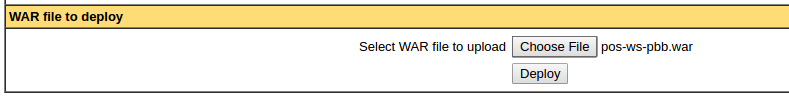
\includegraphics[width=1\textwidth]{./resources/001-deploy-war}
    \caption{\textit{Deploy file} \texttt{war}}
    \label{fig:deploy-war}
  \end{figure}
  
  \item Melakukan pengujian dengan melakukan akses ke \textit{server} menggunakan \textit{browser}, seperti terlihat pada gambar \ref{fig:ws-worked} :
  
  \begin{figure}[H]
    \centering
    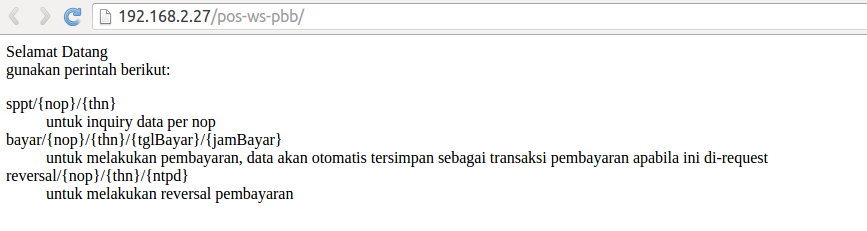
\includegraphics[width=0.8\textwidth]{./resources/002-ws-worked}
    \caption{Akses ke \textit{Web Services} Sudah Siap}
    \label{fig:ws-worked}
  \end{figure}
  
  \item Selesai.
\end{enumerate}


\section{PETUNJUK PEMAKAIAN}

Seperti terlihat pada halaman awal dari layanan \textit{web services}. Tiga layanan yang ditawarkan, yaitu \textit{inquiry} data, pencatatan pembayaran, dan \textit{reversal} pembayaran dapat dilakukan dengan perintah melalui URL \textit{web}.

Untuk mempermudah pemahaman, karena bentuknya hanya berupa \textit{web service} maka hanya akan 2 (dua) informasi yang dibutuhkan, yaitu berupa \textit{request} dan respon atau dalam kata lain \textit{input} dan \textit{output}. Berikut penjelasan lengkapnya :

\subsection{INPUT}

\textit{Request} yang pertama adalah untuk \textit{inquiry} data tagihan, format dari \textit{inquiry} data ini adalah sebagai berikut :

\begin{lstlisting}
/sppt/{nop}/{thn}
\end{lstlisting}

Dimana \texttt{nop} nantinya diganti dengan Nomor Objek Pajak (NOP) yang diinginkan dan \texttt{thn} digantikan dengan tahun pajak yang diinginkan.

Untuk perintah yang kedua adalah \textit{request} untuk pencatatan pembayaran, perintahnya adalah sebagai berikut :

\begin{lstlisting}
/bayar/{nop}/{thn}/{tglBayar}/{jamBayar}
\end{lstlisting}

Untuk \texttt{nop} nantinya digantikan dengan Nomor Objek Pajak yang diinginkan, untuk \texttt{thn} digantikan dengan tahun pajak yang akan dibayarkan, untuk \texttt{tglBayar} digantikan dengan tanggal terjadinya pembayaran, dan untuk \texttt{jamBayar} digantikan dengan jam saat terjadinya pembayaran.

Untuk perintah yang ketiga adalah \textit{request reversal} pembayaran bila terjadi kesalahan pembayaran.

\subsection{OUTPUT}

\end{document}